\chapter{Module \module{connector}}
\label{connector}

This module provides classes for connecting two \class{box}-instances with
lines, arcs or curves. All constructors of the following connector-classes take
two \class{box}-instances as the two first arguments. They return a connecting
path from the first to the second box. The overall geometry of the path is such
that is starts/ends at the boxes' centers. It is then cut by the boxes'
outlines. The resulting \class{connector} will additionally be shortened by
lengths given in the \keyword{boxdists}-keyword (a list of two lengths, default
\code{[0,0]}).

Angle keywords can be either absolute or relative. The absolute angles refer to
the angle between x-axis and the running tangent of the connector, while the
relative angles are between the direct connecting line of the box-centers and
the running tangent (see figure.~\ref{fig:connector}).

The bulge-keywords parameterize the deviation of the connector from the
connecting line. It has different meanings for different connectors (see
figure.~\ref{fig:connector}).

\section{Class \class{line}}

The constructor of the \class{line} class accepts only boxes and the
\keyword{boxdists}-keyword.

\section{Class \class{arc}}

The constructor takes either the \keyword{relangle}-keyword or a
combination of \keyword{relbulge} and \keyword{absbulge}. The ``bulge'' is
meant to be a hint for the greatest distance between the connecting arc and the
straight connection between the box-centers. (Default: \code{relangle=45},
\code{relbulge=None}, \code{absbulge=None})\smallskip

Note that the bulge-keywords override the angle-keyword.

If both \keyword{relbulge} and \keyword{absbulge} are given, they will be
added.

\section{Class \class{curve}}

The constructor takes both angle- and bulge-keywords. Here, the bulges are
used as distances between the control points of the cubic Bezi\'er-curve.
For the signs of the angle- and bulge-keywords refer to figure~\ref{fig:connector}.

\keyword{absangle1} or \keyword{relangle1}\\
\keyword{absangle2} or \keyword{relangle2}, where the absolute angle overrides the
relative if both are given. (Default: \code{relangle1=45},
\code{relangle2=45}, \code{absangle1=None}, \code{absangle2=None})\medskip

\keyword{absbulge} and \keyword{relbulge}, where they will be added if both are
given.\\ (Default: \code{absbulge=None}, \code{relbulge=0.39}; these default
values produce output similar to the defaults of \class{arc}.)\medskip


\begin{figure}[hbt]
\centerline{
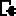
\includegraphics{connector}
}
\caption{The angle-parameters of the connector.arc (left panel) and the
connector.curve (right panel) classes.}
\label{fig:connector}
\end{figure}

\section{Class \class{twolines}}

This class returns two connected straight lines. There is a vast variety of
combinations for angle- and length-keywords. The user has to make sure to
provide a non-ambiguous set of keywords:\medskip

\keyword{absangle1} or \keyword{relangle1} for the first angle,\\
\keyword{relangleM} for the middle angle and\\
\keyword{absangle2} or \keyword{relangle2} for the ending angle.
Again, the absolute angle overrides the relative if both are given. (Default:
all five angles are \code{None})\medskip

\keyword{length1} and \keyword{length2} for the lengths of the connecting lines.
(Default: \code{None})


